\documentclass[10pt,twocolumn,letterpaper]{article}

\usepackage[margin=0.75in]{geometry}
\usepackage[T1]{fontenc}
\usepackage[utf8]{inputenc}
\usepackage{lmodern}
\usepackage{microtype}
\usepackage{graphicx}
\usepackage{xcolor}
\usepackage{hyperref}
\usepackage{amsmath,amssymb,amsthm}
\usepackage{booktabs}
\usepackage{caption}
\usepackage{subcaption}
\usepackage{flushend}
\usepackage{enumitem}
\usepackage{dblfloatfix}
\usepackage{tikz}
\usetikzlibrary{automata,positioning,arrows.meta}

\title{Robot Ping-Pong Control Under Physics Variation:\\
Domain Randomization and Residual Reinforcement Learning}
\author{
Julia Novick\thanks{All authors contributed equally to this work.} \quad Jonathan Zhang \quad Mayand Gulati \quad Sagnik Biswas\\[4pt]
\normalsize UC Santa Barbara
}
\date{March 12, 2026}

\newtheorem{definition}{Definition}
\newtheorem{assumption}{Assumption}
\newtheorem{proposition}{Proposition}
\newtheorem{remark}{Remark}

\hypersetup{
  colorlinks=true,
  linkcolor=blue!70!black,
  citecolor=blue!70!black,
  urlcolor=blue!70!black,
  breaklinks=true
}

\begin{document}
\raggedbottom
\maketitle

\begin{abstract}
We present a theory-oriented study of residual reinforcement learning for robotic ping-pong under uncertain simulation physics. The controller combines a finite-state-machine and inverse-kinematics baseline (FSM+IK) with a learned Soft Actor-Critic (SAC) residual that provides bounded joint-space corrections. We compare nominal SAC training on fixed physics against robust SAC training with per-episode domain randomization over mass, friction, restitution, and dissipation parameters. Experiments use 20-episode deterministic evaluations at checkpoints (500k, 750k, 1M) under nominal and randomized test physics. Nominal SAC achieves strongest absolute performance (482 mean hits nominal; 328 randomized), while robust SAC exhibits better relative robustness trends at later checkpoints (+25.9\% at 750k and +48.5\% at 1M from nominal to randomized evaluation). We provide SAC theory background, implementation-level design analysis, quantitative results, failure-mode analysis, and reproducibility details. Code and artifacts are public at \url{https://github.com/MG-05/ping-pong-domain-randomization}.
\end{abstract}

\section{Introduction}
Dynamic table-tennis control is a challenging robotic benchmark because high-frequency contact events amplify small model errors. In this project, policy quality is not determined solely by nominal return; it is also determined by resilience under physically plausible perturbations. This motivates a robustness-first framing.

Our system uses a hybrid architecture:
\begin{itemize}[leftmargin=*,noitemsep]
    \item an analytic inner loop (FSM+IK) for structured intercept and strike behavior,
    \item a learned residual outer loop (SAC) for corrective adaptation.
\end{itemize}

This decomposition supports a rigorous question: when does residual learning improve performance, and how does domain randomization change generalization behavior?

We evaluate three research questions:
\begin{itemize}[leftmargin=*,noitemsep]
    \item \textbf{RQ1 (Absolute Performance):} Can residual SAC exceed the hand-engineered baseline?
    \item \textbf{RQ2 (Robustness):} Does domain-randomized training improve behavior under perturbed physics?
    \item \textbf{RQ3 (Stability):} What do variance and survival metrics reveal about policy reliability?
\end{itemize}

\section{Related Work}
\textbf{Entropy-regularized RL.}
SAC optimizes return plus policy entropy, giving strong continuous-control performance and improved training stability~\cite{haarnoja2018sac}.

\textbf{Continuous-control actor-critic lineage.}
Deterministic actor-critic methods such as DDPG~\cite{lillicrap2015ddpg} show the utility of off-policy replay-based learning in robotics, but can be brittle under noise and hyperparameter shifts.

\textbf{Domain randomization.}
Randomizing simulator dynamics can reduce overfitting to a single simulator instance and improve out-of-distribution robustness~\cite{tobin2017domainrand,peng2018sim2real}.

\textbf{Robust and residual RL.}
Robust RL emphasizes performance under perturbations~\cite{pinto2017robust}; residual RL combines structured control priors with learned corrections for safety and sample efficiency~\cite{johannink2019residualrl}.

\textbf{Practical implementation framework.}
Stable-Baselines3 provides reproducible, standard RL training infrastructure that we leverage for SAC training and evaluation orchestration~\cite{raffin2021sb3}.

\section{Theoretical Background}
\subsection{MDP and Residual Action Parameterization}
Let \(\mathcal{M}=(\mathcal{S},\mathcal{A},P,r,\gamma)\) denote the control process~\cite{sutton2018rl}.
Here, \(s_t\in\mathbb{R}^{20}\) contains robot and ball state, and \(a_t\in[-1,1]^7\) is a normalized residual action.

Baseline and residual are combined as
\[
q_t^{\mathrm{cmd}}
=\Pi_{\mathcal{Q}}\!\left(q_t^{\mathrm{base}}+\alpha\delta\,\mathrm{clip}(a_t,-1,1)\right),
\]
where \(\alpha\) is residual scale, \(\delta\) is max residual magnitude, and \(\Pi_{\mathcal{Q}}\) projects onto joint limits.

\subsection{SAC Objective}
SAC solves an entropy-regularized objective
\[
J(\pi)=\mathbb{E}_{\tau\sim\pi}\left[\sum_{t=0}^{\infty}\gamma^t\left(r_t+\beta\mathcal{H}(\pi(\cdot|s_t))\right)\right].
\]
The soft Bellman operator defines
\begin{align*}
Q^\pi(s_t,a_t) &= r_t+\gamma\,\mathbb{E}\!\left[V^\pi(s_{t+1})\right], \\
V^\pi(s) &= \mathbb{E}_{a\sim\pi}\!\left[Q^\pi(s,a)-\beta\log\pi(a|s)\right].
\end{align*}

\subsection{Why Residual SAC Is Appropriate for This Task}
Robot ping-pong involves known geometric structure (intercept timing and IK). Learning full control from scratch is unnecessary and increases exploration burden. Residual SAC addresses a narrower problem: improving a feasible baseline policy via bounded corrections.

\begin{proposition}[Residual boundedness]
If \(q_t^{\mathrm{base}}\in\mathcal{Q}\), then \(q_t^{\mathrm{cmd}}\in\mathcal{Q}\) for all \(t\).
\end{proposition}
\textit{Proof sketch:} \(q_t^{\mathrm{cmd}}\) is explicitly projected by \(\Pi_{\mathcal{Q}}\).

\begin{remark}
This boundedness ensures residual exploration cannot directly violate joint-position constraints.
\end{remark}

\subsection{Robustness Under Transition Shift}
Let \(P_{\mathrm{nom}}\) and \(P_{\mathrm{rand}}\) denote nominal and randomized transition kernels. Training only on \(P_{\mathrm{nom}}\) may maximize nominal return while degrading under \(P_{\mathrm{rand}}\). Domain-randomized training approximates risk minimization over a distribution of perturbations.

\subsection{SAC Training Dynamics in Residual Control}
For this project, SAC optimization is best interpreted as learning a correction distribution over a moving baseline controller output. Unlike standard end-to-end policy learning, the action semantics are locally corrective: each action dimension perturbs one joint around a feasible IK-informed command. This affects critic learning in two ways.

First, replay buffer support is naturally concentrated around physically plausible commands, because the baseline controller prevents extreme off-manifold states. Second, value approximation error can still accumulate due to contact discontinuities (ball-paddle impacts), leading to the non-monotonic checkpoint behavior observed in our results.

In actor-critic form, SAC alternates:
\begin{itemize}[leftmargin=*,noitemsep]
    \item \textbf{critic updates}: regress soft Bellman targets under replayed transitions;
    \item \textbf{actor updates}: maximize soft value while preserving entropy;
    \item \textbf{target updates}: Polyak averaging controlled by \(\tau\).
\end{itemize}
Because the reward combines sparse event terms (new hit) and dense shaping terms (alive/apex), critic targets mix abrupt and smooth components. This mixed structure plausibly contributes to temporary value-function mismatch at intermediate checkpoints.

\subsection{Entropy Temperature and Exploration Interpretation}
In SAC, entropy regularization controls exploration intensity. In a residual-control setting, higher entropy does not mean arbitrary behavior in task space; it means diverse local perturbations around structured baseline commands. This can be advantageous when baseline timing is approximately correct but contact quality requires adaptation.

However, entropy-driven exploration can still produce transiently suboptimal residual patterns before converging to better correction strategies. The 500k \(\rightarrow\) 750k dip followed by 1M rebound in both nominal and robust tracks is consistent with such reorganization.

\subsection{Critic and Actor Losses (Conceptual Form)}
In implementation terms, SAC alternates stochastic gradient steps on:
\begin{align*}
\mathcal{L}_Q(\phi) &=
\mathbb{E}_{(s,a,r,s')\sim\mathcal{D}}
\left[\left(Q_\phi(s,a)-y(r,s')\right)^2\right],\\
y(r,s') &= r + \gamma\left(
\min_{i\in\{1,2\}}Q_{\bar\phi_i}(s',a')
 - \beta\log\pi_\theta(a'|s')
\right),
\end{align*}
with \(a'\sim\pi_\theta(\cdot|s')\). The actor objective is:
\[
\mathcal{L}_\pi(\theta)=
\mathbb{E}_{s\sim\mathcal{D},a\sim\pi_\theta}
\left[\beta\log\pi_\theta(a|s)-\min_i Q_{\phi_i}(s,a)\right].
\]
These objectives are not re-derived in code, but they are the optimization principles inherited from the SAC implementation used by Stable-Baselines3.

\subsection{Distributional Robustness Perspective}
Let \(\xi\) denote randomized physics parameters (mass, friction, restitution, dissipation) sampled from distribution \(\mathcal{P}_\Xi\). Nominal training approximates:
\[
\max_\pi \; \mathbb{E}_{\tau\sim P_{\xi_0},\pi}[R(\tau)],
\]
while robust training approximates:
\[
\max_\pi \; \mathbb{E}_{\xi\sim\mathcal{P}_\Xi}\mathbb{E}_{\tau\sim P_{\xi},\pi}[R(\tau)].
\]
This does not guarantee worst-case optimality, but it better aligns optimization with deployment where physics are uncertain.

\begin{proposition}[Expected-risk interpretation]
If test-time dynamics are sampled from \(\mathcal{P}_\Xi\), then robust-domain-randomized training is an unbiased Monte Carlo estimator of expected return under that distribution (up to function-approximation error and finite sample effects).
\end{proposition}

\textit{Practical implication:}
robust SAC can improve average behavior across perturbations even when it does not maximize peak nominal performance.

\section{Methods and Implementation}
\subsection{Environment and Timing}
The environment (\texttt{src/envs/residual\_env.py}) runs physics at \(1\) ms and applies RL control at \(10\) ms. This time-scale separation preserves contact fidelity while keeping policy inference tractable.

\subsection{Observation, Action, and Interfaces}
\textbf{Observation (20-D):}
\[
o_t=[q_{1:7},\dot{q}_{1:7},p_b^x,p_b^y,p_b^z,v_b^x,v_b^y,v_b^z].
\]
\textbf{Action (7-D):}
normalized residual in \([-1,1]^7\), mapped to bounded joint offsets.

At each control step:
\begin{enumerate}[leftmargin=*,noitemsep]
    \item evaluate FSM+IK to get \(q_t^{\mathrm{base}}\),
    \item compute residual-corrected command,
    \item apply to plant input,
    \item advance simulator by control interval.
\end{enumerate}

\subsection{Reward Construction}
Reward includes:
\begin{itemize}[leftmargin=*,noitemsep]
    \item alive bonus when ball remains above minimum height,
    \item hit bonus for debounced contact events,
    \item apex-tracking bonus \(r_{\mathrm{apex}}\exp(-10\cdot e_{\mathrm{apex}}^2)\),
    \item drop penalty on terminal failure.
\end{itemize}

This design balances persistence, contact productivity, and bounce quality.

\subsection{Training Configuration}
From \texttt{src/train\_rl.py}, SAC is configured with:
\begin{itemize}[leftmargin=*,noitemsep]
    \item MLP policy \([256,256]\),
    \item learning rate \(3\times10^{-4}\),
    \item batch size 256,
    \item replay buffer 100k,
    \item \(\gamma=0.99\), \(\tau=0.005\),
    \item residual scale \(0.5\), max residual \(0.15\) rad.
\end{itemize}

Two training tracks are used:
\begin{itemize}[leftmargin=*,noitemsep]
    \item \textbf{Nominal SAC:} fixed dynamics.
    \item \textbf{Robust SAC:} randomized dynamics on each reset.
\end{itemize}

\subsection{Domain Randomization Mechanism}
\texttt{src/utils/randomization.py} samples parameters from the ranges in Table~\ref{tab:dr_ranges} and writes randomized model/scenario files before each robust episode.

\begin{table}[t]
\centering
\caption{Domain randomization ranges used in robust training.}
\label{tab:dr_ranges}
\small
\begin{tabular}{lcc}
\toprule
Parameter & Min & Max \\
\midrule
Ball mass (kg) & 0.0020 & 0.0035 \\
Ball friction & 0.15 & 0.30 \\
Ball restitution & 0.85 & 0.95 \\
Paddle mass (kg) & 0.08 & 0.15 \\
Paddle friction & 0.20 & 0.60 \\
Paddle restitution & 0.80 & 1.00 \\
Floor dissipation & 0.01 & 0.10 \\
Floor restitution & 0.80 & 1.00 \\
\bottomrule
\end{tabular}
\end{table}

\section{Experimental Protocol}
\subsection{Hypotheses}
\begin{itemize}[leftmargin=*,noitemsep]
    \item \textbf{H1:} Residual SAC can exceed FSM baseline hit counts.
    \item \textbf{H2:} Domain-randomized SAC improves relative perturbation robustness.
    \item \textbf{H3:} Learning dynamics are non-monotonic across checkpoints.
\end{itemize}

\subsection{Evaluation Procedure}
\texttt{src/evaluate.py} runs deterministic policy inference for 20 episodes per model-condition pair.
Evaluated checkpoints: 500k, 750k, 1M.
Evaluated conditions: nominal and randomized physics.

\subsection{Metrics}
\begin{definition}[Mean hit performance]
For episode hits \(h_e\), \(H=\frac{1}{N}\sum_{e=1}^{N}h_e\).
\end{definition}

\begin{definition}[Relative perturbation effect]
\[
\Delta(\%)=100\cdot\frac{H_{\mathrm{rand}}-H_{\mathrm{nom}}}{H_{\mathrm{nom}}}.
\]
\end{definition}

\begin{definition}[Relative variability]
\[
\mathrm{CV}(\%)=100\cdot\frac{\sigma_{\mathrm{rand}}}{H_{\mathrm{rand}}}.
\]
\end{definition}

\begin{assumption}[Controlled comparisons]
Within each evaluation block, horizon, deterministic inference mode, and episode count are fixed.
\end{assumption}

\section{Implementation Walkthrough (Conceptual)}
\subsection{End-to-End Dataflow}
At runtime, one control iteration follows this sequence:
\begin{enumerate}[leftmargin=*,noitemsep]
    \item read simulator outputs: iiwa state, ball state, and ball contact-force proxy;
    \item evaluate the FSM controller to generate \(q_t^{\mathrm{base}}\);
    \item query residual SAC policy for normalized action \(a_t\);
    \item map \(a_t\) to bounded joint corrections and add to \(q_t^{\mathrm{base}}\);
    \item clamp to joint bounds and apply position command to the station;
    \item advance simulation by one control interval and compute reward/termination.
\end{enumerate}
This decomposition isolates high-level tactical behavior (intercept/strike logic) from low-level adaptation (residual correction), making failures easier to diagnose than in monolithic policies.

\subsection{Why the Observation Space Is Structured This Way}
The 20-D observation contains joint position/velocity and ball position/velocity. Conceptually, this is the minimum state needed to:
\begin{itemize}[leftmargin=*,noitemsep]
    \item infer arm configuration and motion trend,
    \item infer ball flight state for near-term intercept correction,
    \item avoid overfitting to simulator-internal artifacts.
\end{itemize}
No image stream is used; this keeps the problem in a dynamics-control regime rather than perception-heavy policy learning.

\subsection{Reward Design Trade-offs}
The reward blends sparse success events and dense shaping:
\begin{itemize}[leftmargin=*,noitemsep]
    \item sparse hit bonuses produce strong task signal but can destabilize critic learning when contacts are rare;
    \item alive and apex shaping terms reduce reward sparsity but may create local optima (e.g., keeping short rallies alive rather than maximizing long-term hit count);
    \item drop penalties discourage catastrophic failure but can overweight terminal events if improperly tuned.
\end{itemize}
In this project, the combined reward appears effective for discovering high-hit trajectories at 1M, but also exhibits checkpoint volatility, suggesting potential future reward-scaling work.

\subsection{Contact Event Debouncing and Measurement Semantics}
Hit counting uses force-thresholded contact with cooldown debouncing. This matters for interpretation: ``hits'' are not simply every physics-step contact, but filtered events intended to approximate meaningful paddle-ball interactions. Therefore, reported hit-rate differences can reflect both policy behavior and event-definition sensitivity, a point we include in validity threats.

\subsection{Training Infrastructure and Reproducibility}
The training loop uses a standard set of RL engineering controls:
\begin{itemize}[leftmargin=*,noitemsep]
    \item checkpoint callback for temporal model snapshots,
    \item eval callback for periodic deterministic policy evaluation,
    \item monitor-wrapped environments for episodic metrics,
    \item fixed seeds to improve experiment repeatability.
\end{itemize}
This scaffolding is crucial in graduate-level projects because it enables post-hoc analysis of dynamics such as the 750k dip.

\subsection{Domain Randomization as Scenario Generation}
Randomization is implemented by sampling parameters and writing randomized model/scenario files used at environment reset. This means perturbations alter actual simulation artifacts (not merely internal coefficients) and better reflect realistic structural variation in contact dynamics.

\subsection{FSM Controller Architecture}
The baseline controller is a six-state finite state machine (Figure~\ref{fig:fsm_diagram}) implemented in \texttt{src/controllers/fsm\_controller.py}. Each state maps to a distinct phase of the ping-pong rally cycle:

\begin{itemize}[leftmargin=*,noitemsep]
    \item \textbf{WAIT}: holds the home joint configuration; monitors ball state for planning conditions (ball descending, above minimum height, cooldown expired).
    \item \textbf{PLAN}: predicts a ballistic intercept at the target hit height (\(0.38\) m), computes desired paddle pose and normal, and solves IK for three waypoints (prehit, hit, follow-through). Transitions to PREHIT on success or RECOVER on failure.
    \item \textbf{PREHIT}: interpolates the arm from its current configuration toward the prehit waypoint. May replan if time permits. Transitions to STRIKE at the scheduled strike start time.
    \item \textbf{STRIKE}: executes a timed linear interpolation through prehit\(\to\)hit\(\to\)follow waypoints. Detects contact via force threshold or ball velocity reversal.
    \item \textbf{FOLLOW\_THROUGH}: holds the follow-through pose briefly (\(\sim\!0.10\) s), then returns to WAIT.
    \item \textbf{RECOVER}: returns to home pose when planning fails or a strike is missed; transitions to WAIT once joint position and velocity are within tolerance of home.
\end{itemize}

\begin{figure}[t]
\centering
\resizebox{\columnwidth}{!}{%
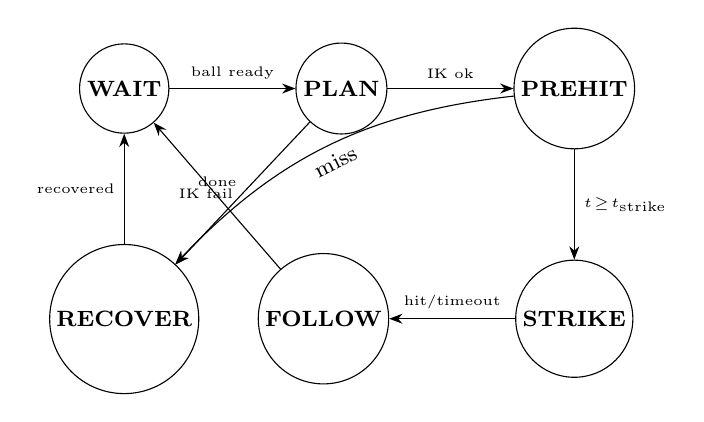
\begin{tikzpicture}[
    ->,>=Stealth,
    node distance=1.4cm and 1.6cm,
    every state/.style={draw,rounded corners,minimum size=0.7cm,font=\footnotesize\bfseries,inner sep=2pt},
    every edge/.append style={font=\tiny}
]
\node[state] (W) {WAIT};
\node[state,right=of W] (P) {PLAN};
\node[state,right=of P] (PH) {PREHIT};
\node[state,below=of PH] (S) {STRIKE};
\node[state,left=of S] (FT) {FOLLOW};
\node[state,below=of W] (R) {RECOVER};

\path (W)  edge node[above]{ball ready} (P)
      (P)  edge node[above]{IK ok} (PH)
      (P)  edge node[left]{IK fail} (R)
      (PH) edge node[right]{$t\!\ge\!t_{\mathrm{strike}}$} (S)
      (PH) edge[bend right=20] node[below,sloped]{\footnotesize miss} (R)
      (S)  edge node[above]{hit/timeout} (FT)
      (FT) edge node[above]{done} (W)
      (R)  edge node[left]{recovered} (W);
\end{tikzpicture}%
}
\caption{FSM state diagram for the baseline controller. Transitions are driven by ball tracking, IK feasibility, timing schedules, and contact detection.}
\label{fig:fsm_diagram}
\end{figure}

This FSM contributes three structural priors that benefit residual learning: a \emph{trajectory feasibility prior} (IK-generated targets keep the arm in physically meaningful postures), a \emph{temporal prior} (strike windows are aligned with predicted intercept timing), and a \emph{contact prior} (the controller encodes an intended paddle-ball contact geometry). As a result, residual SAC learns \emph{how to improve} an already competent policy rather than learning table tennis from scratch.

\subsection{Inverse Kinematics Solver}
The IK stage within PLAN uses Drake's optimization-based \texttt{InverseKinematics} solver to convert Cartesian strike targets into feasible joint configurations. For each strike, the planner solves IK sequentially for three waypoints: prehit (approach pose), hit (contact pose), and follow-through (exit pose), seeding each solve from the previous solution.

The IK program enforces four constraint types:
\begin{enumerate}[leftmargin=*,noitemsep]
    \item \textbf{Joint limits}: bounding-box constraints on all 7 iiwa joints.
    \item \textbf{Seed window}: each joint is constrained within \(\pm 0.65\) rad of the seed configuration, keeping solutions kinematically smooth.
    \item \textbf{Position}: the paddle frame origin must be within \(12\) mm of the target Cartesian point.
    \item \textbf{Orientation}: the paddle normal must be within \(1^\circ\) of the desired strike normal, computed from the incoming ball velocity direction with a tilt gain for directional control.
\end{enumerate}
A quadratic cost penalizes deviation from the seed configuration (weight 2.5 per iiwa joint), biasing solutions toward postures close to the current arm state. If the solver fails to find a feasible solution for any waypoint, the FSM transitions to RECOVER rather than executing an infeasible strike.

\subsection{Why Deterministic Evaluation Is Used}
Evaluation uses deterministic action selection to isolate policy quality from stochastic action sampling noise. This is particularly important when comparing checkpoints, because otherwise performance differences can be confounded by changing policy entropy realization.

However, deterministic evaluation also creates a limitation: under nominal fixed physics, some metrics become near-deterministic (e.g., near-zero standard deviation), reducing visibility into variability. We therefore include randomized evaluation and variance metrics to recover uncertainty information.

\subsection{MuJoCo Sim-to-Sim Transfer}
To test cross-simulator generalization, we evaluate all policies in a MuJoCo reimplementation of the ping-pong environment (\texttt{mujoco\_transfer/}). Table~\ref{tab:mujoco_transfer} reports 500-episode evaluations. Performance drops substantially across the board compared to Drake (Table~\ref{tab:main_results}), confirming that sim-to-sim transfer is nontrivial even when the nominal task geometry is preserved. The FSM baseline achieves 63 mean hits in MuJoCo nominal physics versus 159 in Drake, reflecting contact-model differences between the two simulators. Figure~\ref{fig:mujoco_results} shows the corresponding hit distributions and degradation profiles.

\begin{table}[t]
\centering
\caption{MuJoCo sim-to-sim transfer results (500 episodes per condition).}
\label{tab:mujoco_transfer}
\small
\begin{tabular}{lccc}
\toprule
Model / Physics & Mean Hits & Std & Survival \\
\midrule
FSM Baseline / Nom & 63.0 & 0.0 & 100\% \\
FSM Baseline / Rand & 26.2 & 15.6 & 15.8\% \\
Nominal SAC / Nom & 27.2 & 14.3 & 37.6\% \\
Nominal SAC / Rand & 12.0 & 8.4 & 13.2\% \\
Robust SAC / Nom & 18.6 & 10.4 & 34.4\% \\
Robust SAC / Rand & 13.5 & 8.8 & 22.2\% \\
\bottomrule
\end{tabular}
\end{table}

\begin{figure}[t]
    \centering
    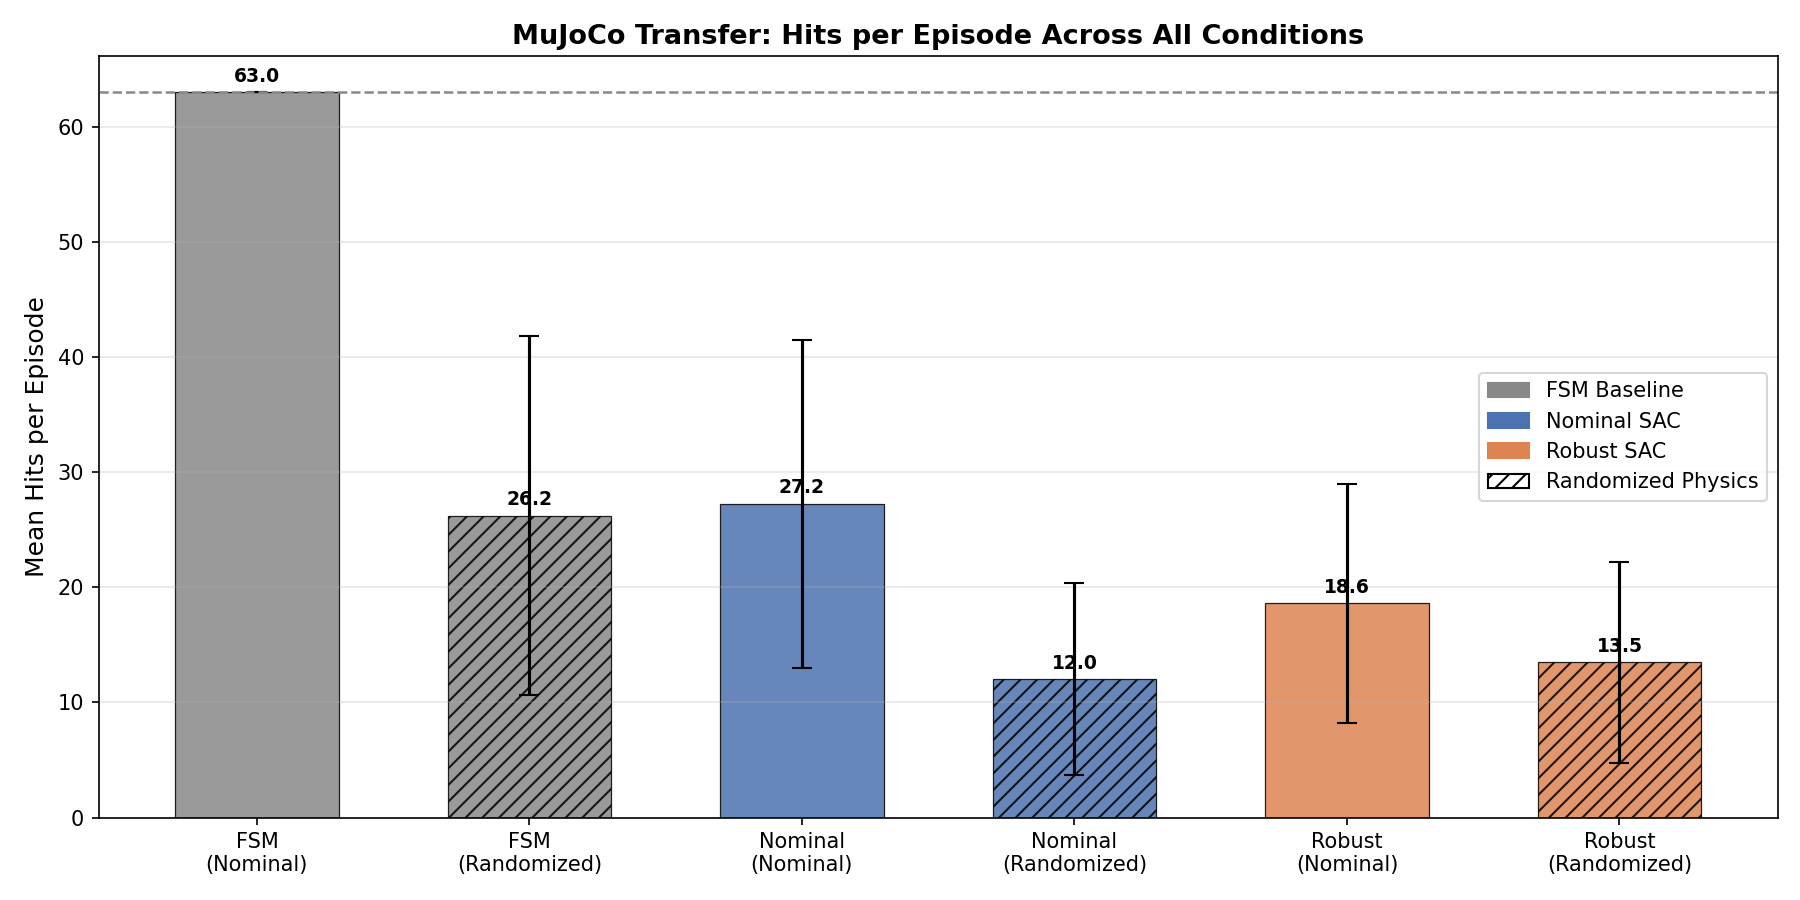
\includegraphics[width=\columnwidth]{results/mujoco_eval_protocol_20260312_155025/hits_comparison.png}
    \caption{MuJoCo sim-to-sim transfer: hit count comparison across models and physics conditions (500 episodes each).}
    \label{fig:mujoco_results}
\end{figure}

\section{Results}
\subsection{FSM Baseline Robustness}
The baseline controller is strong and should not be treated as a trivial reference (Table~\ref{tab:fsm_baseline}).

\begin{table}[t]
\centering
\caption{FSM baseline robustness (dedicated baseline report).}
\label{tab:fsm_baseline}
\small
\begin{tabular}{lcc}
\toprule
Condition & Mean Hits & Full 20 s Survival \\
\midrule
Deterministic init & 154 (single run) & Yes \\
Noisy init (\(\pm\)4 cm) & \(112.3\pm46.7\) & 25/50 (50\%) \\
Stress init (\(\pm\)8 cm) & \(104.3\pm54.9\) & 23/50 (46\%) \\
\bottomrule
\end{tabular}
\end{table}

\subsection{Main Quantitative Comparison}
Table~\ref{tab:main_results} summarizes the full evaluation matrix. Four key findings emerge:

\begin{table*}[t]
\centering
\caption{20-episode evaluation summary across models and physics conditions.}
\label{tab:main_results}
\small
\begin{tabular}{lcccccc}
\toprule
Model & Eval Physics & Mean Hits & Std Hits & Max Hits & Mean Sim Time (s) & \(\Delta\) vs Nominal \\
\midrule
FSM Baseline & Nominal & 159.0 & 0.0 & 159 & 20.0 & -- \\
FSM Baseline & Randomized & 145.3 & 29.0 & 189 & 17.7 & \(-8.6\%\) \\
\midrule
Nominal SAC 500k & Nominal & 144.0 & 0.0 & 144 & 11.0 & -- \\
Nominal SAC 500k & Randomized & 112.8 & 55.1 & 274 & 8.5 & \(-21.7\%\) \\
Nominal SAC 750k & Nominal & 110.0 & 0.0 & 110 & 6.6 & -- \\
Nominal SAC 750k & Randomized & 61.3 & 35.9 & 156 & 3.9 & \(-44.3\%\) \\
Nominal SAC 1M & Nominal & \textbf{482.0} & 0.0 & \textbf{482} & 20.0 & -- \\
Nominal SAC 1M & Randomized & \textbf{328.0} & \textbf{106.0} & \textbf{474} & 13.9 & \(-32.0\%\) \\
\midrule
Robust SAC 500k & Nominal & 53.0 & 0.0 & 53 & 3.5 & -- \\
Robust SAC 500k & Randomized & 43.4 & 11.0 & 66 & 2.8 & \(-18.2\%\) \\
Robust SAC 750k & Nominal & 23.0 & 0.0 & 23 & 1.7 & -- \\
Robust SAC 750k & Randomized & 29.0 & 7.5 & 51 & 1.8 & \(+25.9\%\) \\
Robust SAC 1M & Nominal & 76.0 & 0.0 & 76 & 1.7 & -- \\
Robust SAC 1M & Randomized & 112.9 & 30.9 & 181 & 2.7 & \(+48.5\%\) \\
\bottomrule
\end{tabular}
\end{table*}

\textbf{Finding 1 (Absolute performance):}
Nominal SAC 1M is strongest in raw hit count (Table~\ref{tab:main_results}).

\textbf{Finding 2 (Relative robustness):}
Robust SAC becomes positive in \(\Delta\) at later checkpoints (Figure~\ref{fig:degradation}).

\textbf{Finding 3 (Learning dynamics):}
Both tracks exhibit a 750k dip and 1M rebound (Figure~\ref{fig:learning}).

\textbf{Finding 4 (Consistency):}
Nominal SAC 1M has high randomized variance (\(\sigma=106\)); robust SAC 1M is lower (\(\sigma=30.9\)), as shown in Figure~\ref{fig:variance}.

\subsection{Extended Metric Analysis}
To separate rally quantity from episode duration, we compute mean hit throughput
\(\rho = H / T\), where \(T\) is mean simulation time (Table~\ref{tab:throughput}).

\begin{table}[t]
\centering
\caption{Derived hit throughput (hits/s) from evaluation means.}
\label{tab:throughput}
\small
\begin{tabular}{lcc}
\toprule
Model & Nominal \(\rho\) & Randomized \(\rho\) \\
\midrule
FSM Baseline & 7.95 & 8.23 \\
Nominal 500k & 13.10 & 13.28 \\
Nominal 750k & 16.57 & 15.80 \\
Nominal 1M & 24.10 & 23.60 \\
Robust 500k & 15.19 & 15.25 \\
Robust 750k & 13.37 & 16.05 \\
Robust 1M & 45.24 & 41.50 \\
\bottomrule
\end{tabular}
\end{table}

Table~\ref{tab:throughput} clarifies a subtle behavior: robust policies can exhibit short episodes with very high instantaneous hit throughput (see also Figure~\ref{fig:survival}). Thus, high hit count and long survival are related but not identical objectives in this setup.

\subsection{Checkpoint-by-Checkpoint Interpretation}
\textbf{500k stage.}
Nominal 500k is already competitive with baseline in throughput, while robust 500k remains conservative in absolute hit count. This is consistent with robust training paying an early tax for invariance learning.

\textbf{750k stage.}
Both nominal and robust trajectories dip in nominal evaluation. Robust 750k is notable because randomized performance exceeds nominal performance (\(+25.9\%\)), suggesting adaptation to the randomization distribution even before absolute performance matures.

\textbf{1M stage.}
Nominal 1M undergoes a clear breakthrough in absolute hits under both conditions but retains high OOD variance. Robust 1M improves both mean hits and relative perturbation behavior but still trails nominal 1M in absolute peak.

\subsection{Cross-Metric Tensions}
The results (Figure~\ref{fig:all_results}) expose three objective tensions:
\begin{itemize}[leftmargin=*,noitemsep]
    \item \textbf{Peak hits vs perturbation robustness:} nominal 1M dominates one, robust 1M trends better on the other.
    \item \textbf{Throughput vs episode duration:} some policies hit rapidly in shorter windows.
    \item \textbf{Mean vs predictability:} higher mean can coexist with larger variance.
\end{itemize}

\begin{figure*}[t]
    \centering
    \begin{subfigure}[b]{0.48\textwidth}
        \centering
        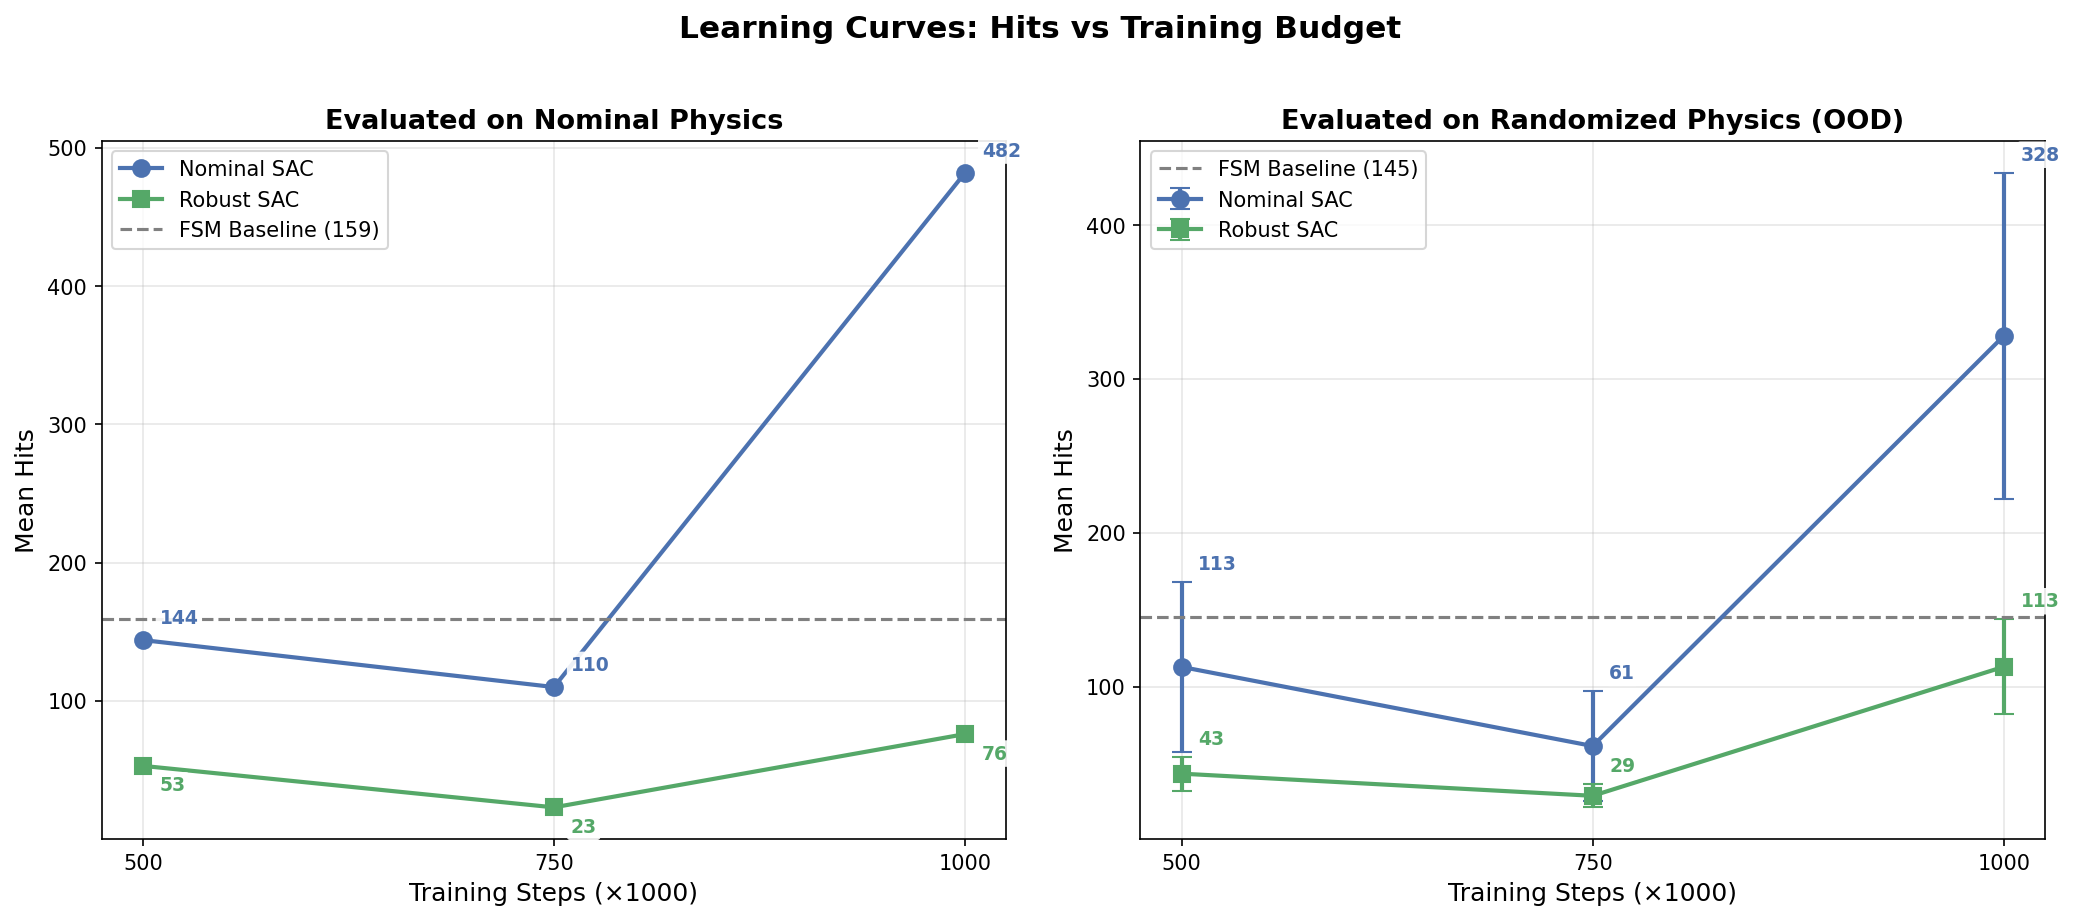
\includegraphics[width=\textwidth]{results/final_learning_curves.png}
        \caption{Learning curves versus training budget.}
        \label{fig:learning}
    \end{subfigure}
    \hfill
    \begin{subfigure}[b]{0.48\textwidth}
        \centering
        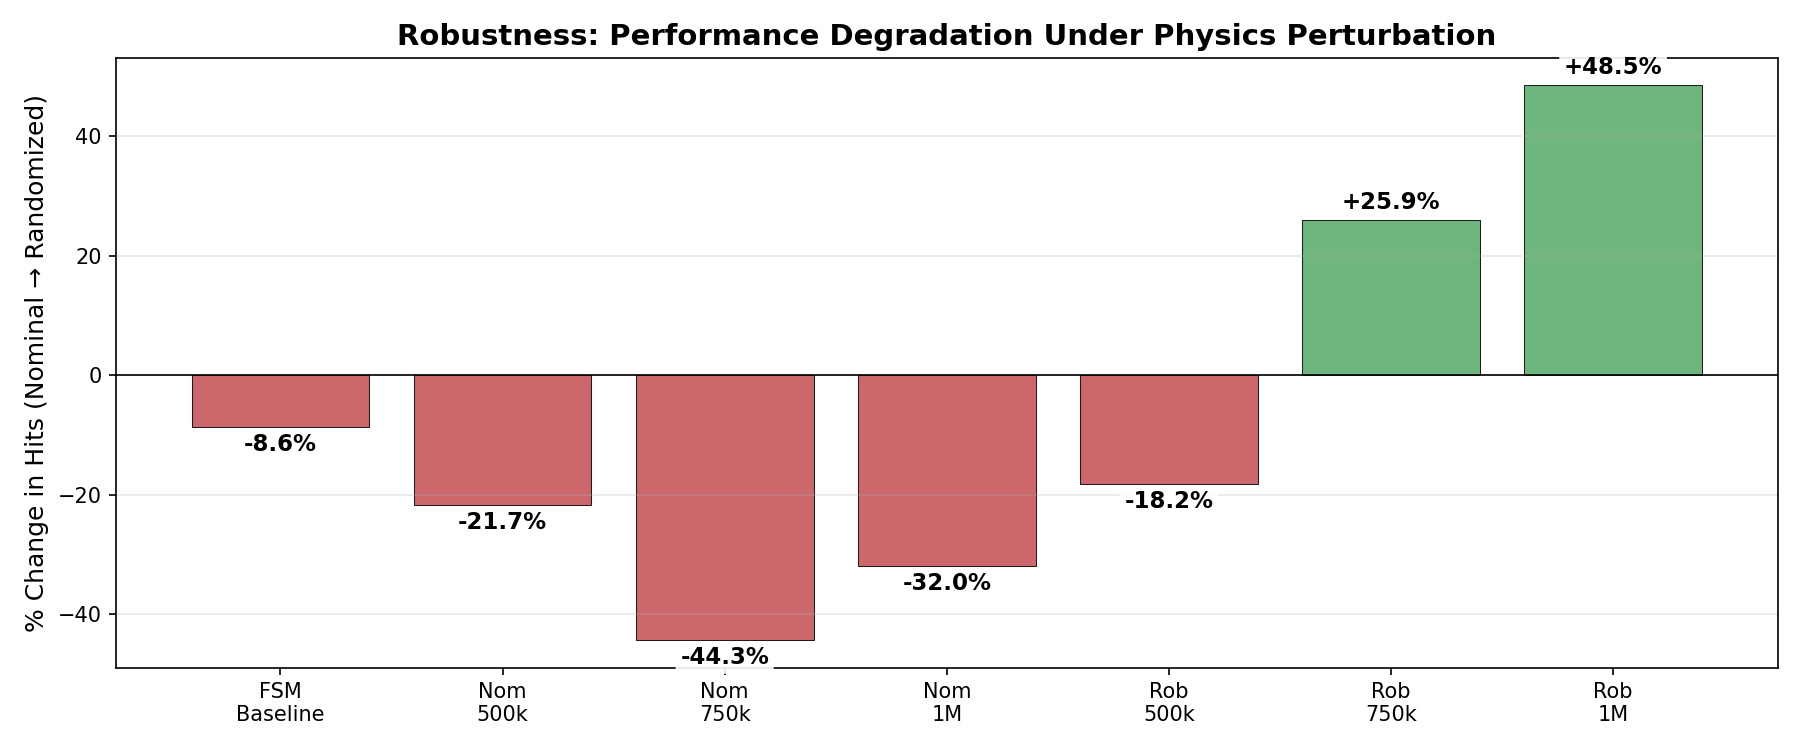
\includegraphics[width=\textwidth]{results/final_degradation.png}
        \caption{Relative perturbation effect \(\Delta\).}
        \label{fig:degradation}
    \end{subfigure}

    \vspace{0.4cm}
    \begin{subfigure}[b]{0.48\textwidth}
        \centering
        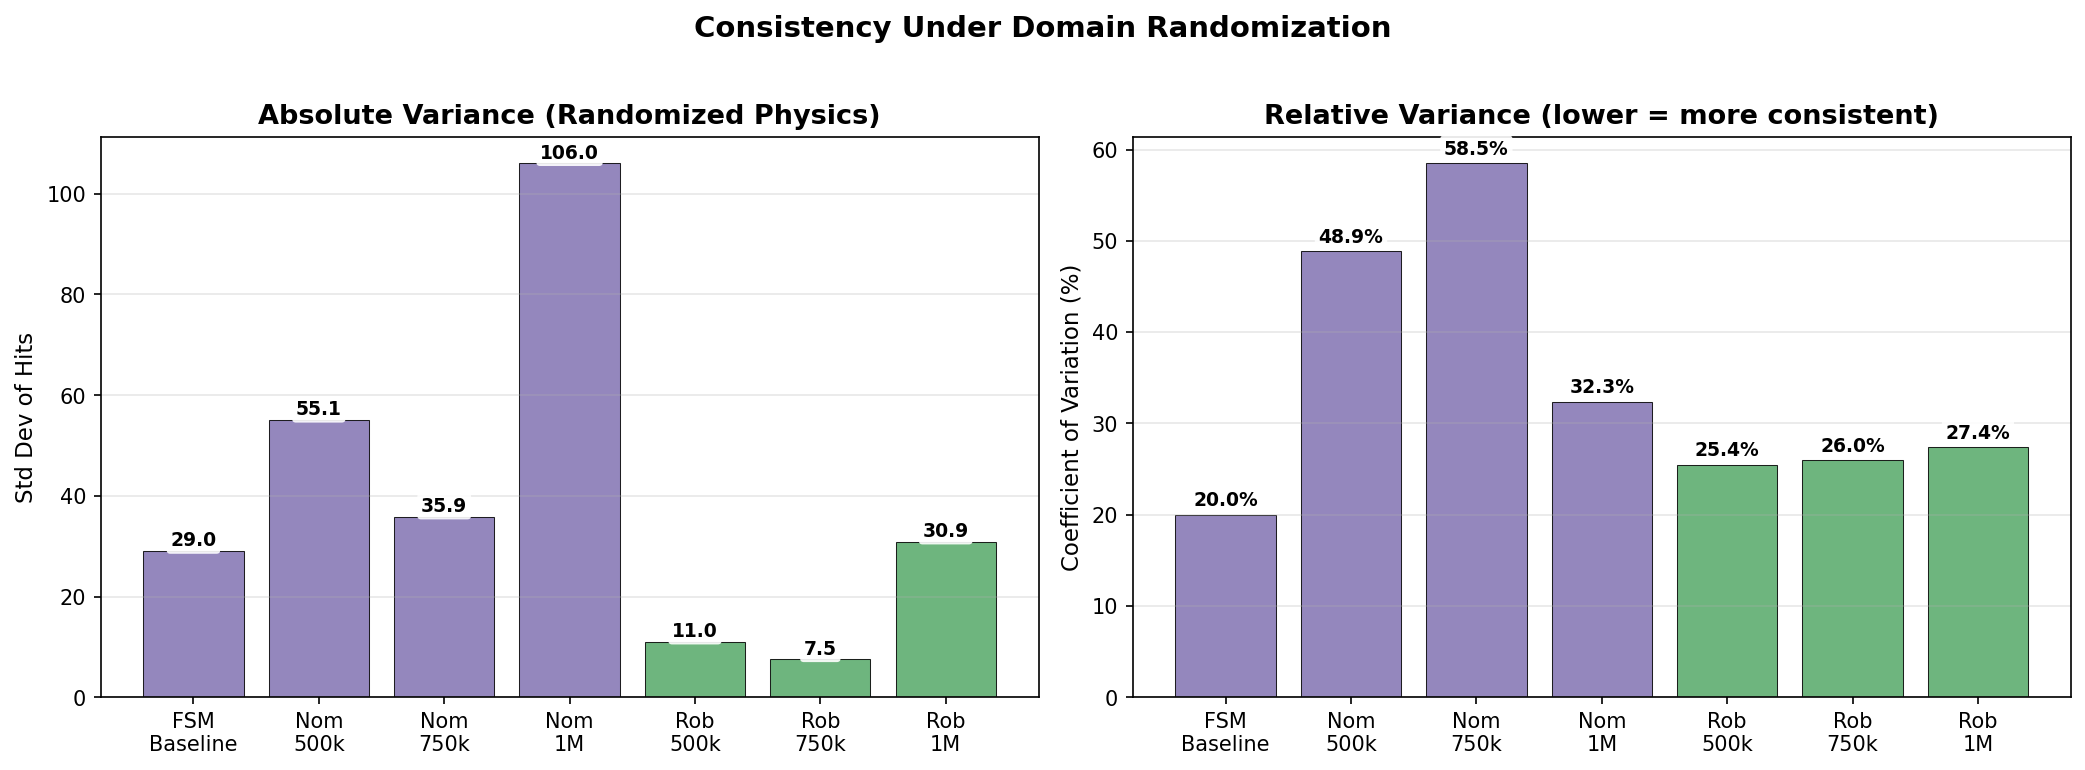
\includegraphics[width=\textwidth]{results/final_variance.png}
        \caption{Absolute and relative variability under randomized physics.}
        \label{fig:variance}
    \end{subfigure}
    \hfill
    \begin{subfigure}[b]{0.48\textwidth}
        \centering
        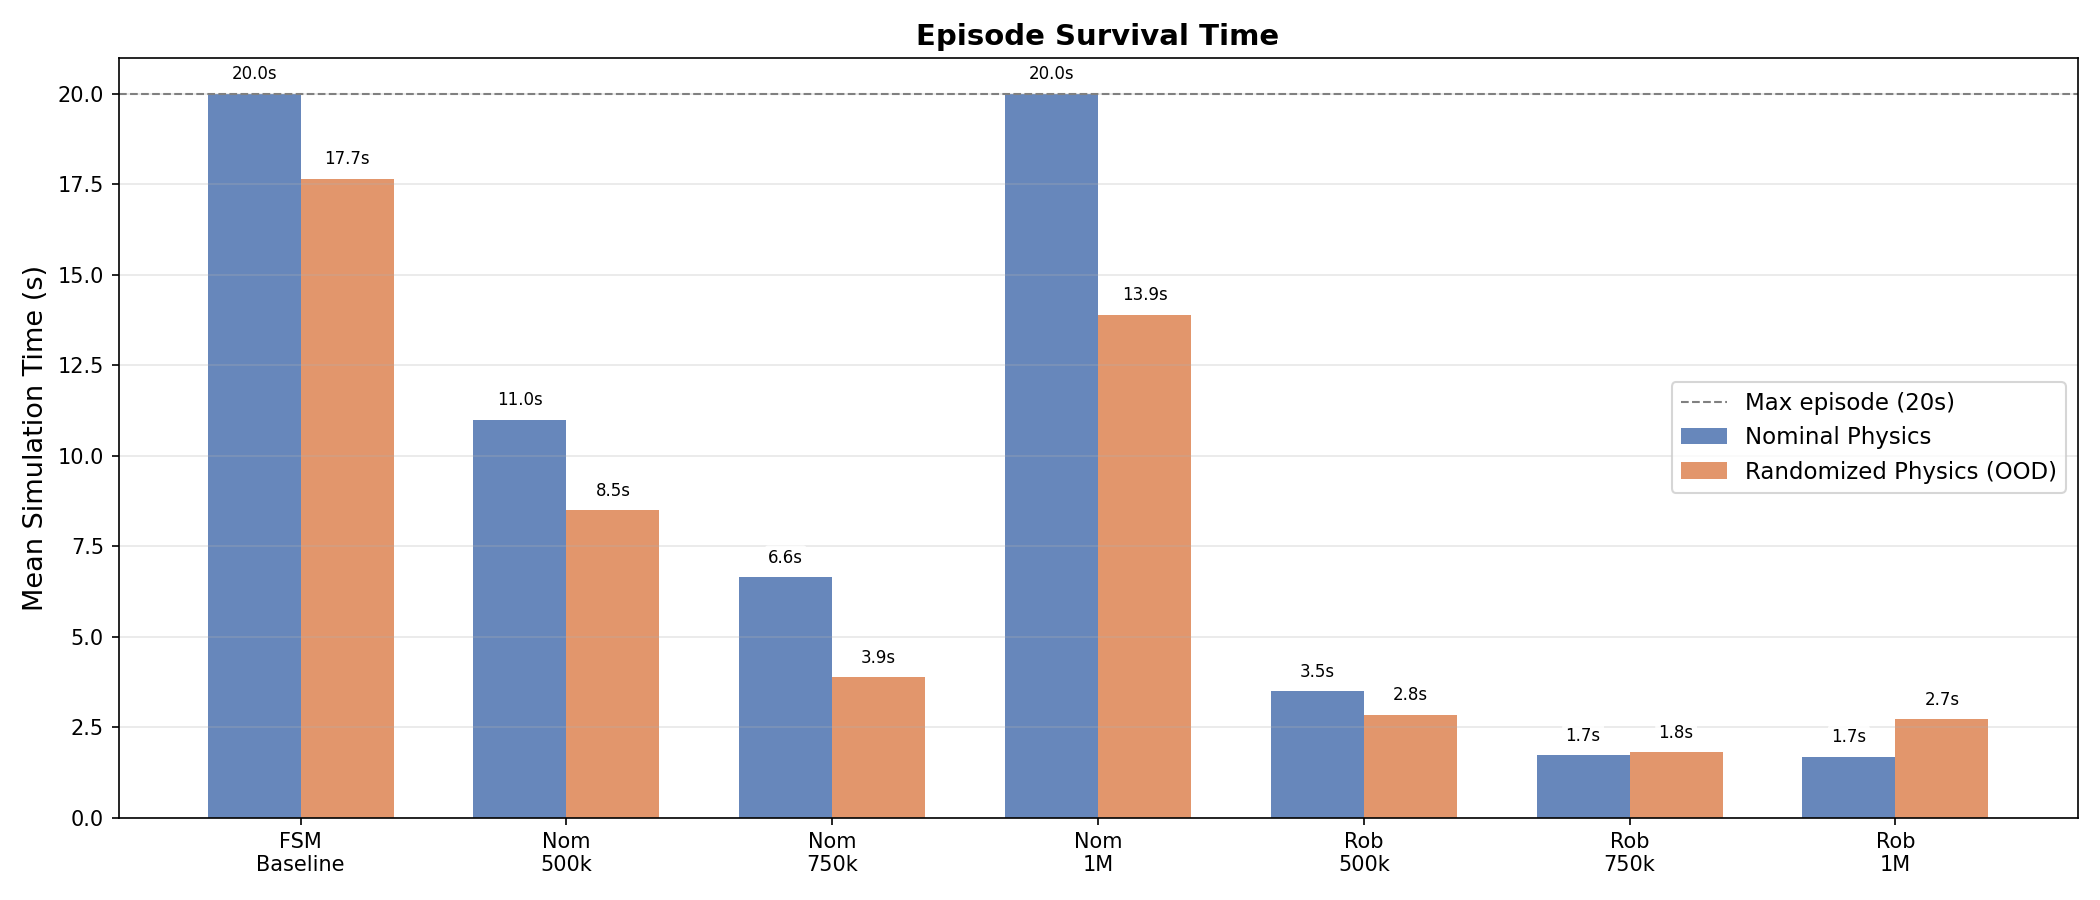
\includegraphics[width=\textwidth]{results/final_survival_time.png}
        \caption{Episode duration comparison.}
        \label{fig:survival}
    \end{subfigure}
    \caption{Core experimental results: performance curves, robustness degradation, variance profiles, and episode survival times across all models and evaluation conditions.}
    \label{fig:all_results}
\end{figure*}

\section{Failure Analysis and Lessons}
The original goal was a single policy that is best in absolute performance and robustness. Under the present budget, this did not happen. Two failure modes emerged:

\textbf{Failure mode A: Nominal over-specialization.}
Nominal SAC learns high-return trajectories but degrades under perturbation (\(-32.0\%\) at 1M). This is consistent with specialization to fixed contact dynamics.

\textbf{Failure mode B: Robust under-optimization.}
Robust SAC improves relative robustness but remains below nominal SAC in peak absolute hits at 1M.

\textbf{Interventions attempted.}
We increased the training budget to 1M and retained intermediate checkpoint evaluation; used wide randomization ranges over contact and inertial parameters; and compared both training types under both evaluation conditions.

\textbf{Interpretation.}
Domain-randomized training appears to allocate capacity toward invariance across physics regimes, which may delay convergence to highly specialized nominal strategies.

\section{Threats to Validity}
\begin{itemize}[leftmargin=*,noitemsep]
    \item \textbf{Single-seed training}: uncertainty across random initializations is not fully characterized.
    \item \textbf{Deterministic nominal evaluation}: near-zero nominal std is expected but limits uncertainty reporting.
    \item \textbf{Simulation-only conclusions}: sim-to-real transfer is not yet validated on hardware.
    \item \textbf{Metric coupling}: hit counting and horizon settings influence rankings.
\end{itemize}

\section{Model-Family Case Analysis}
\subsection{Nominal SAC Family}
The nominal SAC checkpoints illustrate a specialization trajectory. At 500k and 750k, the policy has moderate hit throughput and strong degradation under perturbation. At 1M, the policy reaches a qualitatively different regime with very high hit counts in both nominal and randomized tests, but with substantial variance under randomized physics.

This pattern suggests the learned strategy eventually discovers a high-frequency control mode that strongly exploits nominal simulator structure. The same strategy can still perform well on average under perturbation, but instability increases, consistent with brittle contact sensitivity.

\subsection{Robust SAC Family}
The robust SAC family behaves differently. Early checkpoints are conservative and low in absolute hits, then later checkpoints improve relative perturbation behavior (positive \(\Delta\)). This can be interpreted as the policy gradually internalizing dynamics-invariant corrective behavior.

Although robust 1M underperforms nominal 1M on absolute hit count, it is less volatile under randomized physics. For applications prioritizing reliability under model mismatch, this may be preferable despite lower peak returns.

\subsection{Baseline vs Learned Controllers}
The FSM+IK baseline remains a useful anchor because it is:
\begin{itemize}[leftmargin=*,noitemsep]
    \item interpretable (state-machine phases and IK objectives are inspectable),
    \item stable in nominal deployment,
    \item reasonably robust under moderate perturbation.
\end{itemize}
Residual learning should therefore be judged not only by raw score uplift, but by whether it preserves or improves these baseline reliability properties.

\subsection{Practical Selection Guidance}
Given current evidence, a deployment-oriented selection rule could be:
\begin{itemize}[leftmargin=*,noitemsep]
    \item choose \textbf{Nominal 1M} when maximizing expected throughput in environments close to nominal simulator dynamics;
    \item choose \textbf{Robust 1M} when dynamics uncertainty is large and performance consistency is prioritized;
    \item retain \textbf{FSM+IK} as a fallback safety baseline.
\end{itemize}
This policy-selection framing is often more actionable than a single ``best model'' declaration.

\section{Reproducibility and Experimental Governance}
\subsection{Data Provenance}
The quantitative values in this paper are taken from repository artifacts:
\begin{itemize}[leftmargin=*,noitemsep]
    \item \texttt{results/all\_eval\_results.json}
    \item \texttt{results/fsm\_baseline\_report.md}
    \item \texttt{results/rl\_training\_report.md}
    \item generated figures in \texttt{results/final\_*.png}
\end{itemize}
This provenance path makes each table and plot auditable.

\subsection{Evaluation Integrity Checks}
A graduate-level evaluation should explicitly check:
\begin{itemize}[leftmargin=*,noitemsep]
    \item deterministic-evaluation flag consistency across runs,
    \item checkpoint naming and step-count alignment,
    \item fixed episode count across compared rows,
    \item identical metric definitions (especially hit event detection),
    \item correct mapping between plot labels and table rows.
\end{itemize}
These checks are straightforward but essential for avoiding silent comparison errors.

\subsection{Recommended Reporting Standard}
For stronger final claims, future iterations should report:
\begin{itemize}[leftmargin=*,noitemsep]
    \item multi-seed mean and confidence intervals,
    \item per-episode distributions (not only mean/std aggregates),
    \item sensitivity to reward weights and residual envelope,
    \item additional robustness stress tests beyond current randomization ranges.
\end{itemize}
Even when project goals are only partially met, this reporting standard strengthens scientific credibility and aligns with the syllabus emphasis on rigorous analysis over merely positive outcomes.

\section{Future Directions}
\begin{itemize}[leftmargin=*,noitemsep]
    \item multi-seed confidence intervals for all checkpoints/conditions;
    \item curriculum randomization schedules (narrow-to-wide);
    \item risk-sensitive objectives targeting lower-tail performance;
    \item ablations on residual scale/max residual envelope;
    \item MuJoCo transfer plus real-robot calibration pipeline.
\end{itemize}

\section{Conclusion}
This project demonstrates a rigorous hybrid-control study: residual SAC significantly improves baseline performance, while domain randomization changes robustness behavior in a measurable way. The main scientific outcome is a data-backed trade-off between nominal specialization and perturbation robustness, rather than a single universally dominant policy.

\section*{Code Availability and Reproducibility}
All code, trained models, and evaluation artifacts are publicly available at
\url{https://github.com/MG-05/ping-pong-domain-randomization}.
To reproduce the full experimental pipeline (training, evaluation, and report generation), run the following commands with the repository dependencies installed:

\smallskip
\begin{small}
\begin{verbatim}
python -m src.train_rl --steps 1000000 \
  --no-randomize \
  --save-path data/sac_nominal_1m --seed 42

python -m src.train_rl --steps 1000000 \
  --randomize \
  --save-path data/sac_robust_1m --seed 42

python scripts/run_all_evals.py
python results/generate_final_report.py
\end{verbatim}
\end{small}

\begin{thebibliography}{99}

\bibitem{haarnoja2018sac}
Tuomas Haarnoja, Aurick Zhou, Pieter Abbeel, and Sergey Levine.
\newblock Soft Actor-Critic: Off-Policy Maximum Entropy Deep Reinforcement Learning with a Stochastic Actor.
\newblock In \emph{Proceedings of ICML}, 2018.

\bibitem{lillicrap2015ddpg}
Timothy Lillicrap, Jonathan Hunt, Alexander Pritzel, et al.
\newblock Continuous Control with Deep Reinforcement Learning.
\newblock arXiv:1509.02971, 2015.

\bibitem{tobin2017domainrand}
Josh Tobin, Rachel Fong, Alex Ray, Jonas Schneider, Wojciech Zaremba, and Pieter Abbeel.
\newblock Domain Randomization for Transferring Deep Neural Networks from Simulation to the Real World.
\newblock In \emph{Proceedings of IROS}, 2017.

\bibitem{peng2018sim2real}
Xue Bin Peng, Marcin Andrychowicz, Wojciech Zaremba, and Pieter Abbeel.
\newblock Sim-to-Real Transfer of Robotic Control with Dynamics Randomization.
\newblock In \emph{Proceedings of ICRA}, 2018.

\bibitem{pinto2017robust}
Lerrel Pinto, James Davidson, Rahul Sukthankar, and Abhinav Gupta.
\newblock Robust Adversarial Reinforcement Learning.
\newblock In \emph{Proceedings of ICML}, 2017.

\bibitem{johannink2019residualrl}
Tobias Johannink, Shikhar Bahl, Ashvin Nair, et al.
\newblock Residual Reinforcement Learning for Robot Control.
\newblock In \emph{Proceedings of ICRA}, 2019.

\bibitem{raffin2021sb3}
Antonin Raffin, Ashley Hill, Adam Gleave, et al.
\newblock Stable-Baselines3: Reliable Reinforcement Learning Implementations.
\newblock \url{https://github.com/DLR-RM/stable-baselines3}, 2021.

\bibitem{sutton2018rl}
Richard Sutton and Andrew Barto.
\newblock Reinforcement Learning: An Introduction.
\newblock MIT Press, 2nd edition, 2018.

\end{thebibliography}

\end{document}
